\chapter{Relaxation of integrals of motions in weakly perturbed XXZ model\label{chap:decay}}
\thispagestyle{chapterBeginStyle}


So far we have focused on investigating properties of an \emph{integrable} XXZ
spin-\(1/2\) chain. However, as mentioned in the introductory chapter,
integrability is a rather rare occurrence. Therefore, this chapter is devoted
to the study of (Q)LIOMs in the near-integrable XXZ model. For noncommuting integrals
of motion, we also identity two mechanisms that are at play during the decay of those
observables, namely the integrability breaking itself and the lifting of macroscopic
degeneracy after shifting away from high-symmetry values of anisotropy parameter \(\Delta\).
\textcolor{blue}{Disentanglement of those two processes allows us to explain the origin of anomalous
scaling of relaxation times.}

Methodology in this chapter follows the work of~\textcite{Mierzejewski2015Approx},
however the results about relaxation of noncommuting integrals
of motion are original and at the moment of writing this thesis published as
a preprint~\autocite{mierzejewski2021multiple}.
\section{Adding perturbation to the Hamiltonian}
We are now going to weakly break integrability of XXZ model~\eqref{eq:XXZ} 
by adding a perturbation in form of next-nearest neighbor interaction.
New Hamiltonian has the following form:
\begin{equation}
    H_{XXZ} = \frac{1}{2}\sum_{j = 1}^{L}\left( S^{+}_{j} S^{-}_{j+1} + 
    S^{-}_{j}S^{+}_{j+1} \right) + \Delta\sum_{j = 1}^{L} S^{z}_{j}S^{z}_{j+1}
    + \alpha H^{\prime}
    \label{eq:HXXZ perturbed}
\end{equation}
where \(H'\) is the perturbation that breaks integrability for nonzero \(\alpha \):
\begin{equation}
    H^{\prime}=\sum_{j = 1}^{L} S^{z}_{j}S^{z}_{j+2}
    \label{eq:perturbation}
\end{equation}
In such system, only two conserved quantities remain --- the Hamiltonian \(H_{XXZ}\) itself 
and the total magnetization \(\Sz_{tot}\). All other integrals of motions cease to be conserved
and decay with a finite relaxation time \(\tau\) (cf. Figure~\refeq{fig:cutoff}).
We are interested in investigating this decay and the timescales involved.
To this end we take the previously discussed (Q)LIOMs \(J^E, \hat{O}_1,\hat{O}_2\)
and examine their behavior under finite-time averaging 
(as defined in~\eqref{def:simple time avg}) generated by perturbed Hamiltonian.
As an initial check, we calculate the finite-time autocorrelation function (finite-time stiffness)
\(\lambda^{\tau}_A = \hs{\bar{A}^{\tau}}{\bar{A}^{\tau}}\) as a function of inverse system size.
In order to relate this to the discussion of spectral functions in Section~\ref{sec:spectral function},
we will from now on use the cutoff frequency \(\omega = \frac{1}{\tau}\), instead of the time of
averaging \(\tau\). The perturbation should be strong enough, that in the thermodynamic limit
\(\omega \to 0^+\) stiffness vanishes. Results are shown in Figure~\ref{fig:lioms decay}.
We see first hints that the behavior under perturbation for commuting and noncommuting operators
differ. For perturbation strength \(\alpha=0.2\) energy current stiffness does
not decay in thermodynamic limit for \(\omega \to O^+\) and thus stronger perturbation is needed.
However, stiffness of operators \(\hat{O}_1,\hat{O}_2\) vanish even for finite size systems
and smaller perturbations. 
\textcolor{blue}{Does this make sense? (d)-(i) Increasing nature of
stiffness is caused by \(\omega\) resolution smaller than energy levels spacings? Leave this or
delete this?}.
\begin{figure}[htbp]
  \centering
  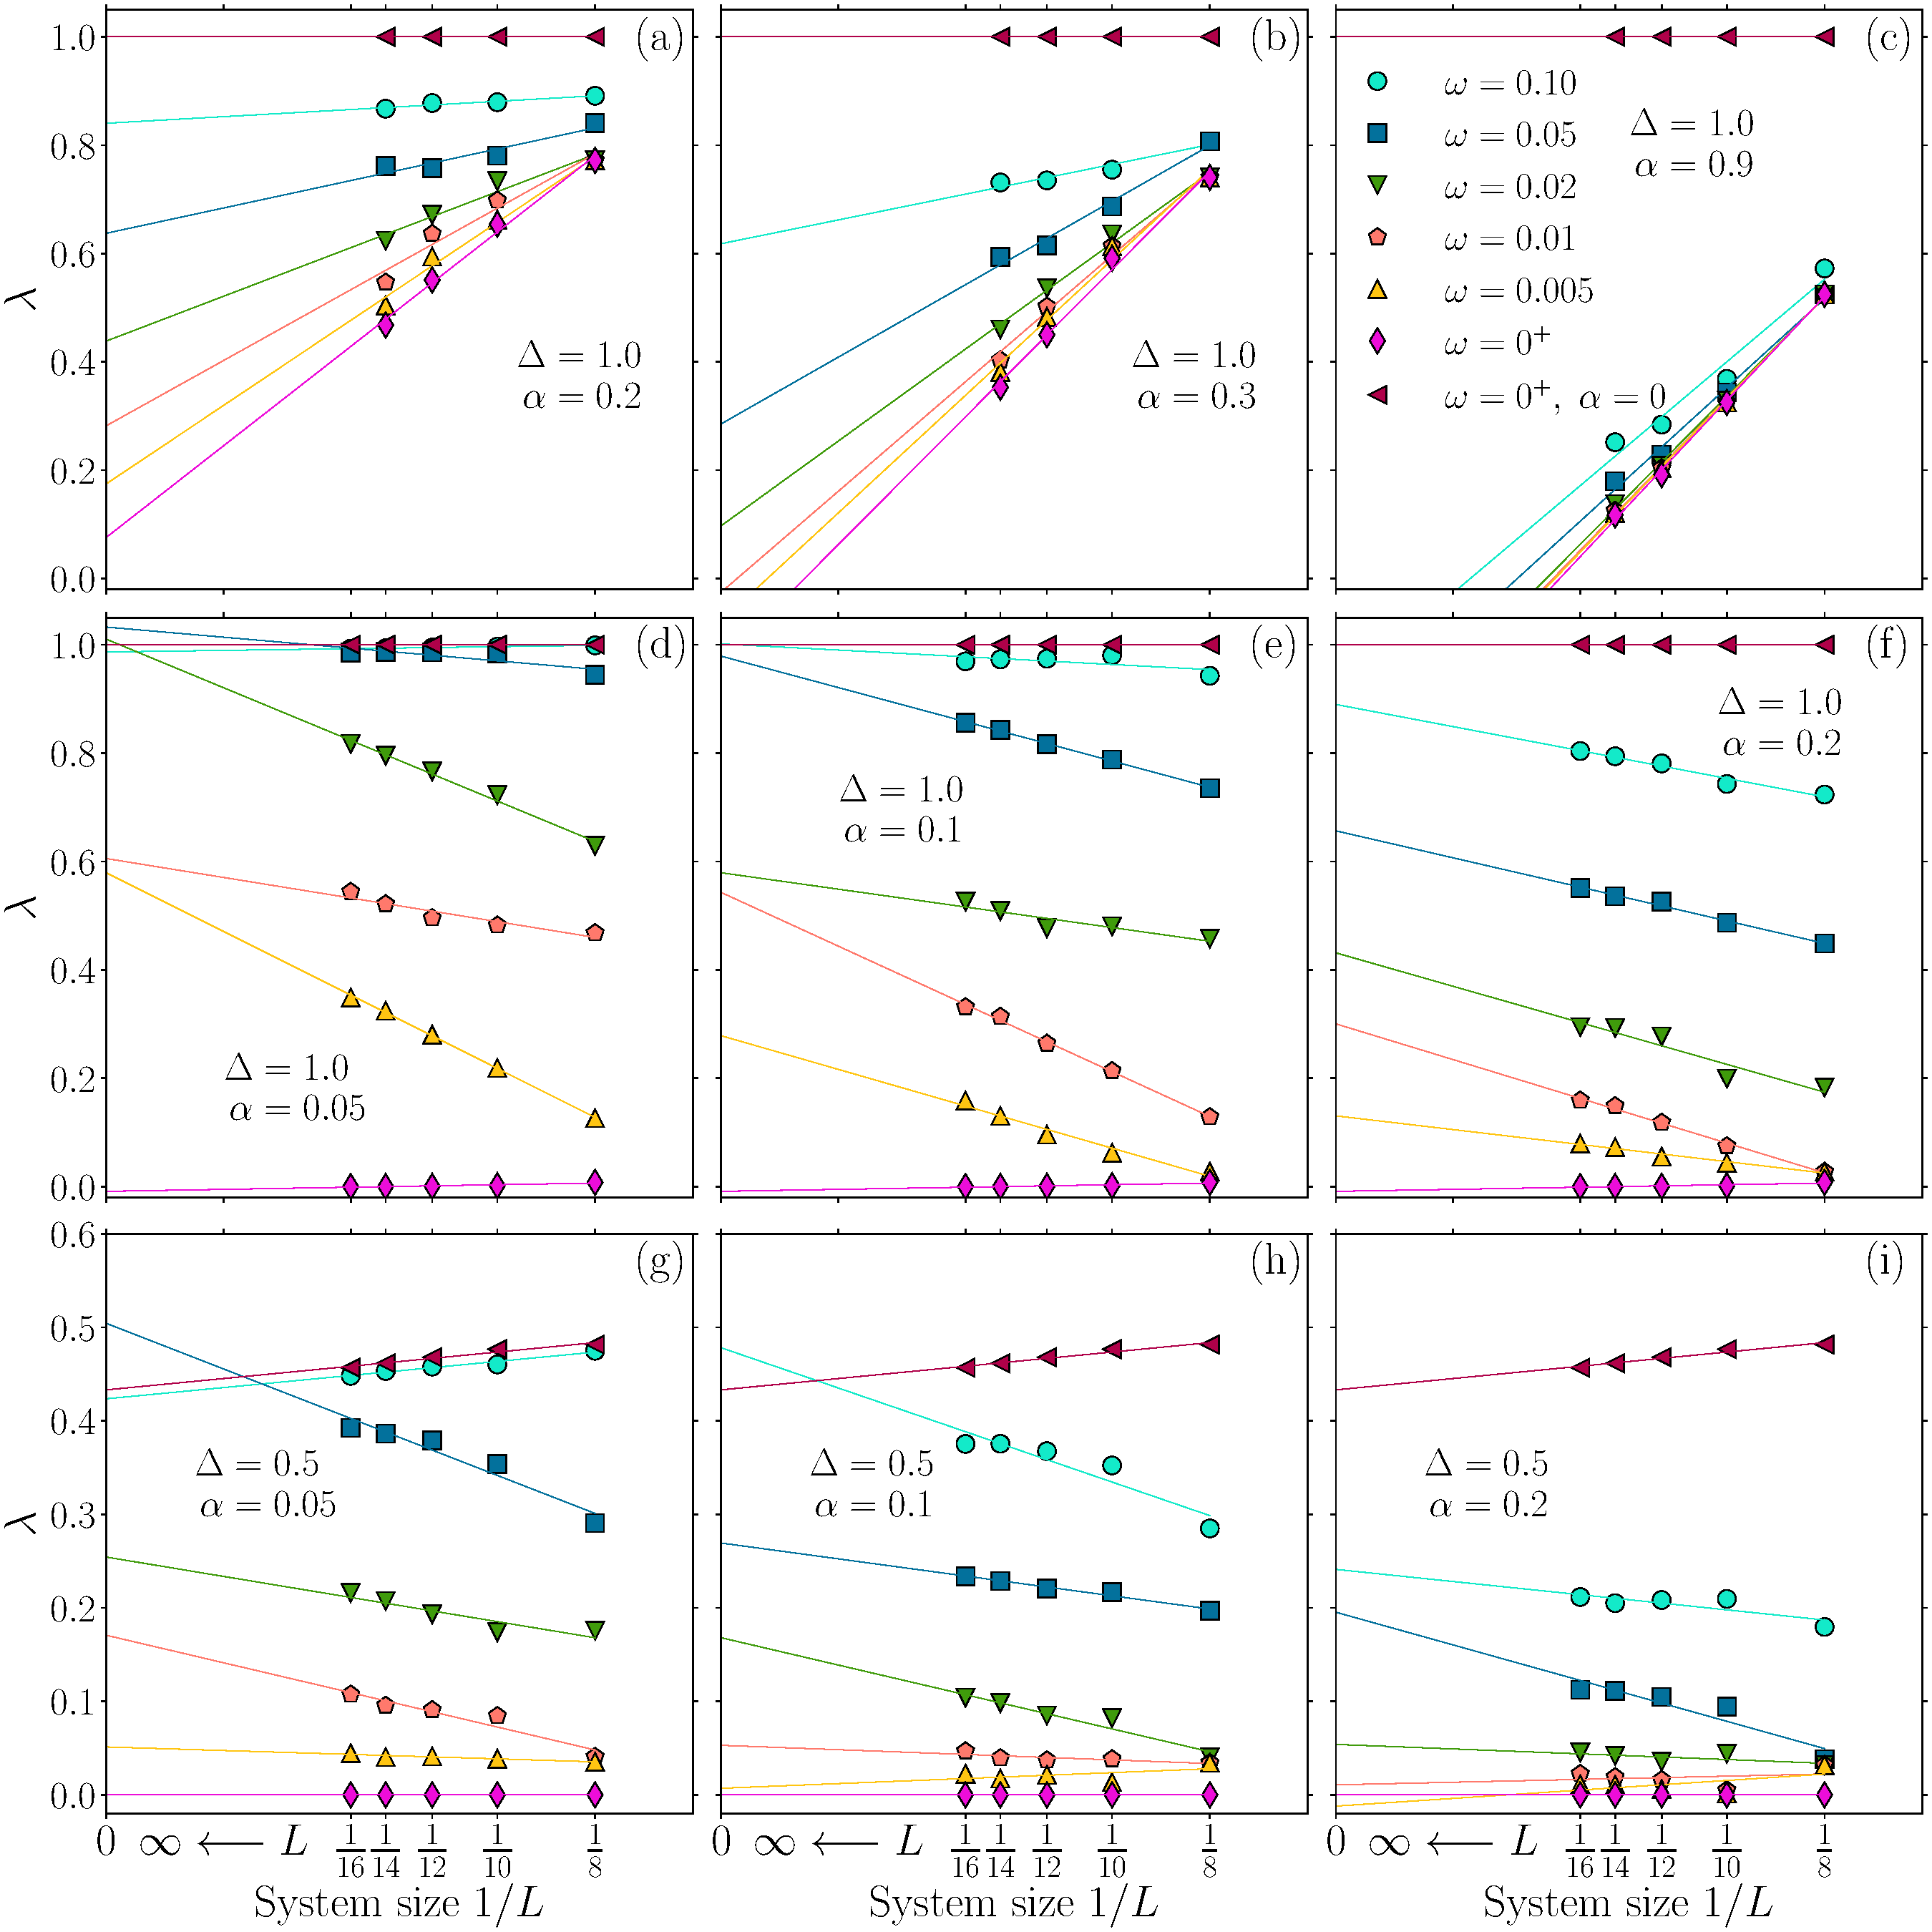
\includegraphics[width=\textwidth]{Figures/lioms_decay.pdf}
  \caption{Finite-time stiffness operators as a function of time for the perturbed Hamiltonian.
  Panels (a)-(c) show results for \(J^E\), (d)-(f) for \(\hat{O}_1\) and (g)-(i) for \(\hat{O}_2\).
  See text for detailed description.}
  \label{fig:lioms decay}
\end{figure}

\newcommand{\figsize}{0.95}
\setlength{\belowcaptionskip}{0pt}
\section{Relaxation of known (Q)LIOMs}
To investigate how our (Q)LIOMs decay with time, we will apply the formalism of spectral functions
described in Sections~\ref{sec:spectral function}.
Since we are interested in the low-\(\omega\) (long times) part of integrated spectral function
\(I(\omega)\), it is convenient to normalize it. Therefore, let us define the
following~\autocite{Mierzejewski2015Approx}:
\begin{equation}
  R_{\hat{A}}(\omega,\alpha) = \frac{I(\omega,\alpha)}{\lim_{\omega \to 0^{+}} I(\omega,\alpha=0)} = 
  \frac{\sum_{n,m}\theta\left(\omega -\abs{E_n-E_m}\right) \abs*{\matrixel{m}{\hat{A}}{n}}^2}
  {\sum_{\substack{n,m \\ E_n=E_m}} \abs*{\matrixel{m}{\hat{A}}{n}}^2}
  \label{eq:normalized integrated spectral function}
\end{equation}
This normalization of \(I(\omega)\) assures that  \(\lim_{\omega\to \infty} R_{\hat{A}}
(\omega,\alpha) = 1\). However at first we should establish a range of values of
parameter \(\alpha\) so its small enough that \(H'\) remains a perturbation but large enough
to be relevant for finite system sizes accessible numerically. As mentioned in previous section,
we are looking vanishing infinite-time stiffness in thermodynamic limit. Therefore, we will
take \(\alpha\) as small as possible so that  \(\lim_{\omega\to 0^{+}} R_{\hat{A}}
(\omega,\alpha) = 0\).

\subsection{Relaxation of energy current}
We begin with the case energy current \(J^E\) for \(\Delta = 1.0\), as derived in Section~\ref{sec:energy current}.
In the integrable parent model it is a conserved quantity, so we have the following:
\begin{equation*}
  \hs{J^E(t)}{J^E} = const \implies S(\omega) \propto \delta(\omega)
  \implies R_{J^E}(\omega,\alpha=0) = 1
\end{equation*}
\begin{figure}[ht]
  \centering
  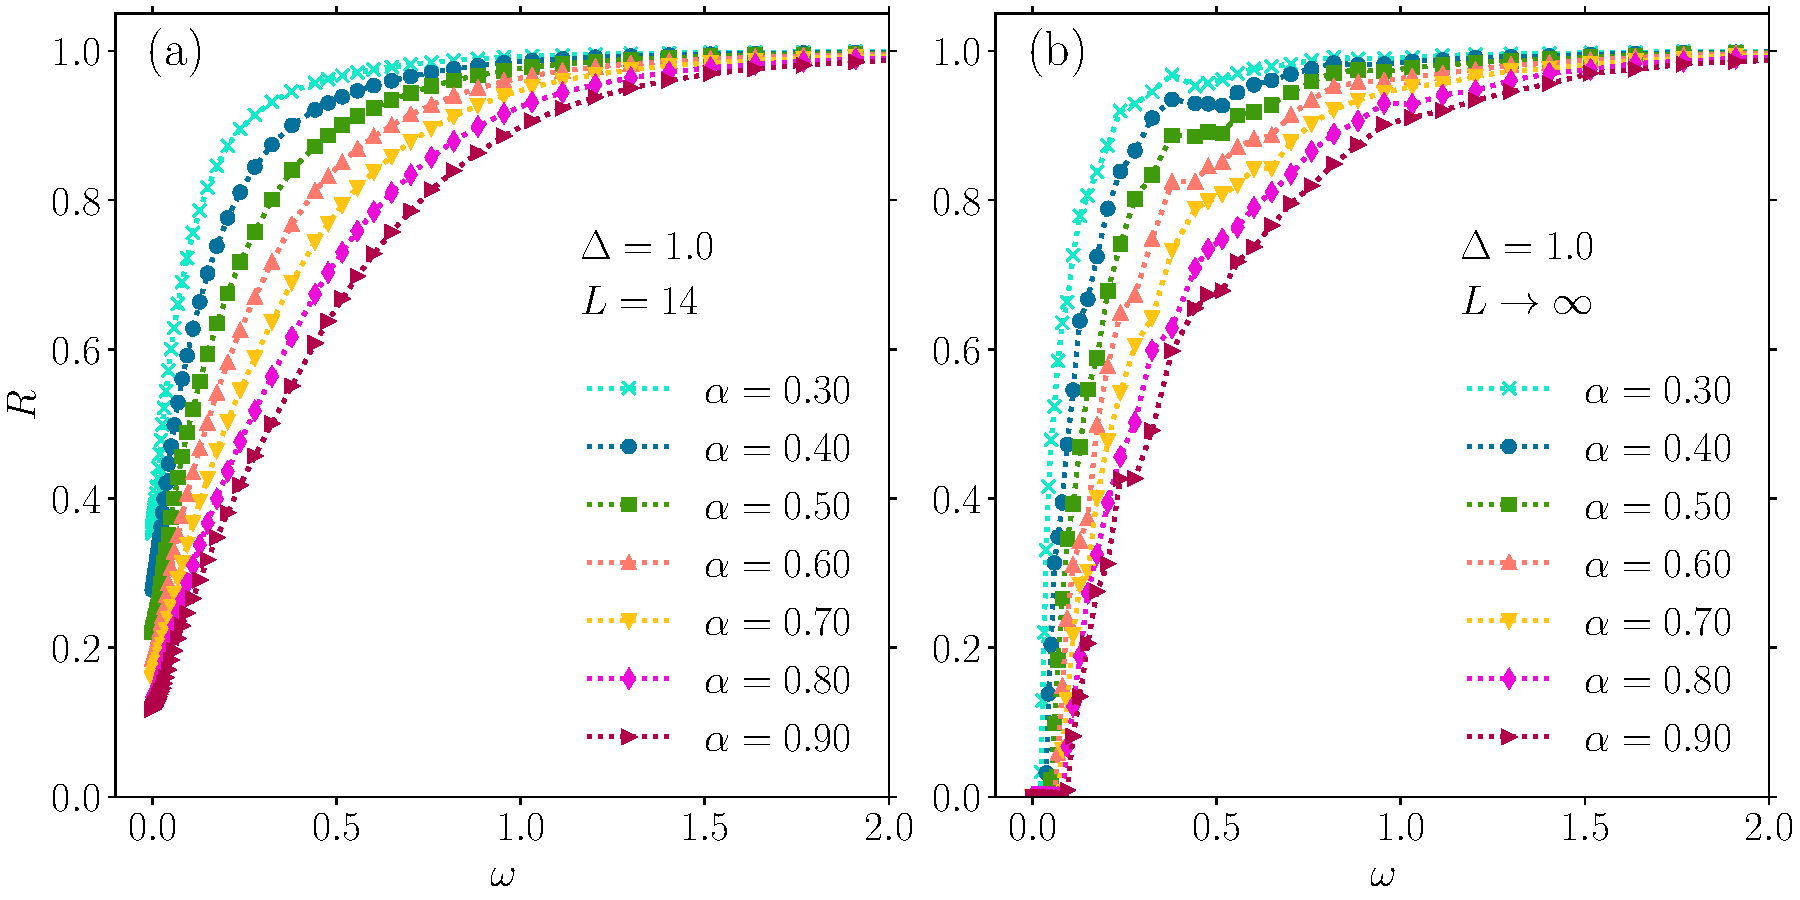
\includegraphics[width=\figsize\textwidth]{Figures/current_no_scaling.pdf}
  \caption{Normalized integrated spectral function as a function of cutoff frequency for \(J^E\).
  (a) Results for \(L=14\). Low frequency limit does not approach 0
  because of finite size effects. (b) Results extrapolated to thermodynamic limit from \(L=11,12,13,14\).
  Note the expected observation, namely stronger perturbation leads to faster decay.}
  \label{fig:current decay no scaling}
\end{figure}
After moving away from integrable regime, the autocorrelation function starts to decay,
so the \(\delta\)-peak broadens and \(R_{J^E}(\omega,\alpha=0)\) is no longer equal to one,
but approaches zero as time increases. We will look simultaneously at two different situations,
results for \(L=14\) and results extrapolated to thermodynamic limit from \(L=11,12,13,14\). 
Figure~\ref{fig:current decay no scaling} shows \(R_{J^E}(\alpha,\omega)\) as a
function of \(\omega\) for \(\alpha=0.3,0.4,0.5\). We immediately see the expected outcome, as the
stronger the perturbation the faster the current decays. The fact that for finite \(L\),
\(R_{J^E}(\alpha,\omega)\) does not approach \(0\) in \(\omega\to 0^+\) limit is consistent
with results in Figure~\ref{fig:lioms decay}.
\begin{figure}[ht]
  \centering
  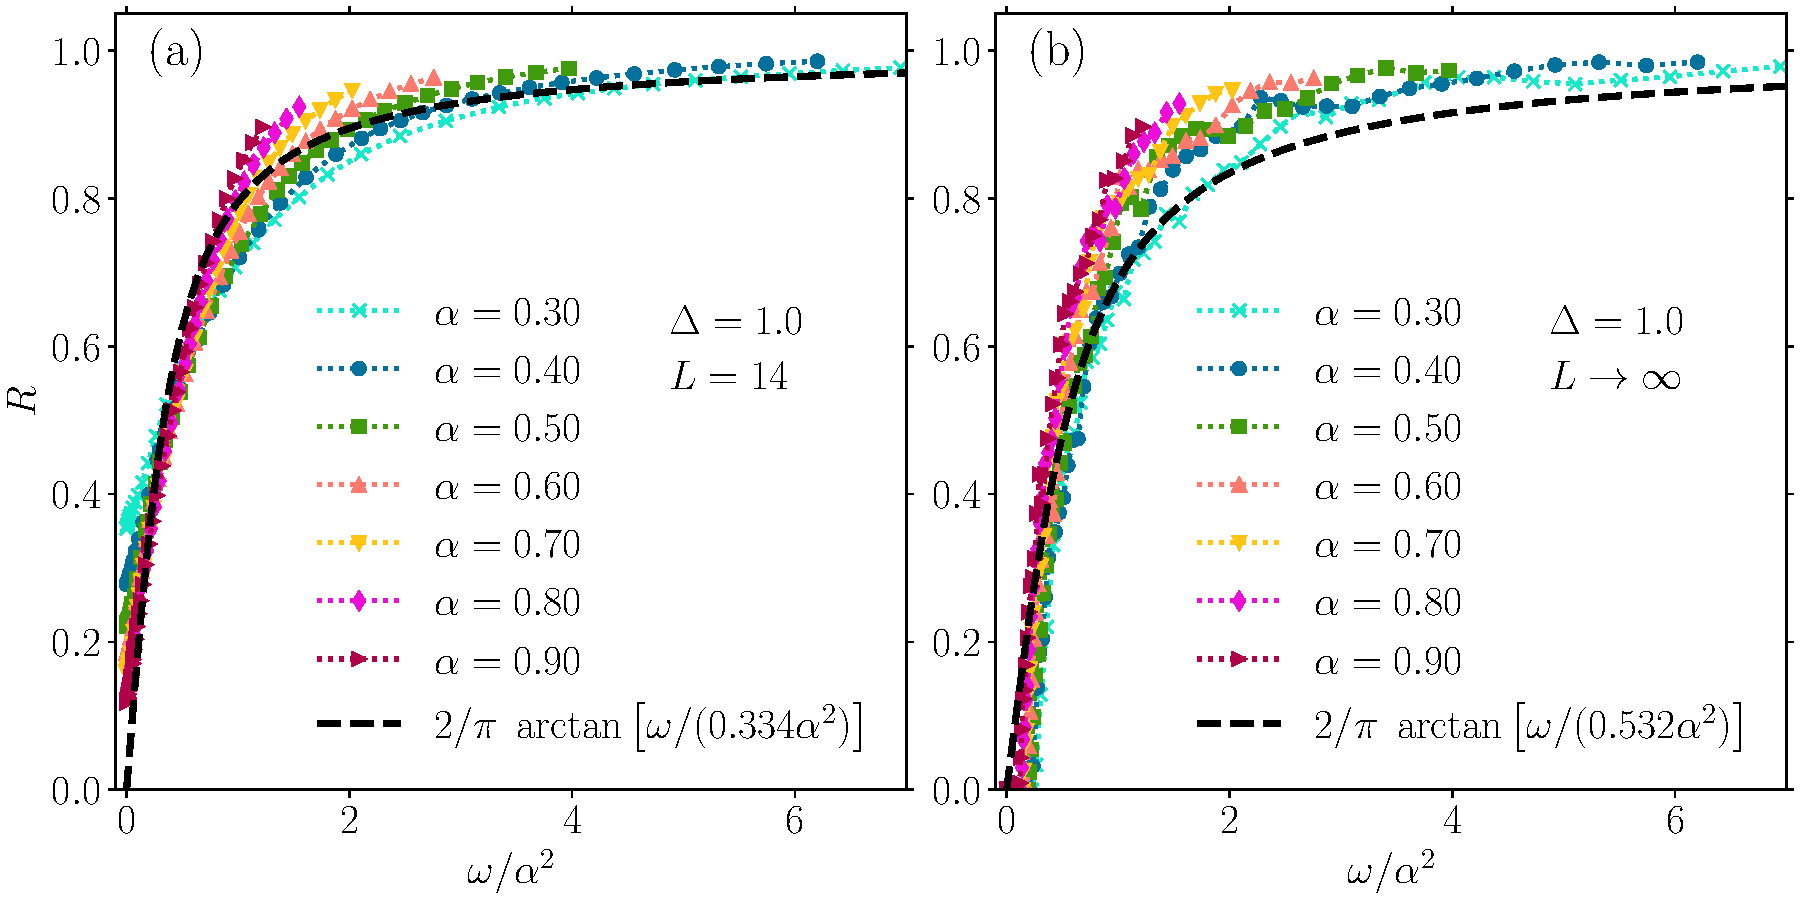
\includegraphics[width=\figsize\textwidth]{Figures/current_scaling.pdf}
  \caption{Normalized integrated spectral function as a function of rescaled cutoff frequency for \(J^E\).
  (a) Results for \(L=14\). (b) Results extrapolated to thermodynamic limit from \(L=11,12,13,14\).
  Dashed black line corresponds to fit~\eqref{eq:R arctan}.}
  \label{fig:current decay scaling}
\end{figure}
However, an interesting thing happens when plot the same data, but as a function of rescaled
frequency \(\omega/\alpha^2\). Numerical results visible on Figure~\ref{fig:current decay scaling}
show a convincing collapse of curves for different values of perturbation strength. This may suggest
an universal dependence of \(R(\omega,\alpha)\) on \(\omega\) and \(\alpha\):
\begin{equation}
  R(\omega,\alpha)\simeq \tilde{R}(\omega/\alpha^2)
  \label{eq:universal scaling current}
\end{equation}
Moreover, this relation can be reasonably well approximation by a one parameter fit
(black dashed line in Figure~\ref{fig:current decay scaling}):
\begin{equation}
  \tilde{R}(\omega/\alpha^2) \simeq \frac{2}{\pi} \arctan\left(\frac{\omega}{\gamma \alpha^2}\right)
\label{eq:R arctan}
\end{equation}
where \(\gamma \) is the fitting parameter. It implies that the relaxation of energy current
is exponential in nature. To see this, let us calculate \(I(\omega)\) for such decay
\(\hs{J^E(t)}{J^E} \propto \mathrm{e}^{-\abs{t}/\tau_{j}}\). Double-sided exponential has well defined Fourier
transform, so we can drop the \(\epsilon \to 0^{+}\) limit from the integral.
\begin{align}
  S(\omega) &\propto \frac{1}{2\pi} \int_{-\infty}^{\infty} \mathrm{d} t\; \mathrm{e}^{-\abs{t}/\tau_{j}} \mathrm{e}^{i \omega t} = 
  \frac{1}{2\pi} \left[\int_{-\infty}^{0} \mathrm{d} t\; \mathrm{e}^{(1/\tau_{j} + i\omega)t }
  + \int_{0}^{\infty} \mathrm{d} t\; \mathrm{e}^{(-1/\tau_{j} + i\omega)t }  \right] \nonumber \\
  &= \frac{1}{2\pi} \left[\frac{\tau_{j}}{1+i\omega \tau_{j}} + \frac{\tau_{j}}{1-i\omega\tau_{j}}\right] = 
  \frac{1}{\pi} \frac{\tau_{j}}{1+\omega^2\tau_{j}^2}
\end{align}
Integrating \(S(\omega)\) over a frequency window we obtain:
\begin{equation*}
  I(\omega) \propto \frac{1}{\pi}\int_{-\omega}^{\omega}\mathrm{d}\omega^{\prime}\; 
  \frac{\tau_{j}}{1+\omega^2\tau_{j}^2} = \frac{2}{\pi} \arctan(\tau_{j} \omega)
\end{equation*}
which after normalization yields the desired results~\eqref{eq:R arctan}. Furthermore, we learn that the 
characteristic relaxation time \(\frac{1}{\tau_{j}} \propto \alpha^2\) and the proportionality
constant is universal and does not depend on \(\alpha\).
The quadratic scaling shown on Figure~\ref{fig:current decay scaling} is actually not the
best possible for this set of numerical data. Choosing the rescaling coefficient to be
\(\frac{3}{2}\) allows for almost perfect collapse of all the curves 
(see Figure~\ref{fig:current decay perfect scaling}). However, it is expected to be a consequence
of working with rather small system sizes, because in was shown 
in~\textcite{Mierzejewski2015Approx} using memory function formalism, that quadratic scaling
is indeed the appropriate one.
\begin{figure}[ht]
  \centering
  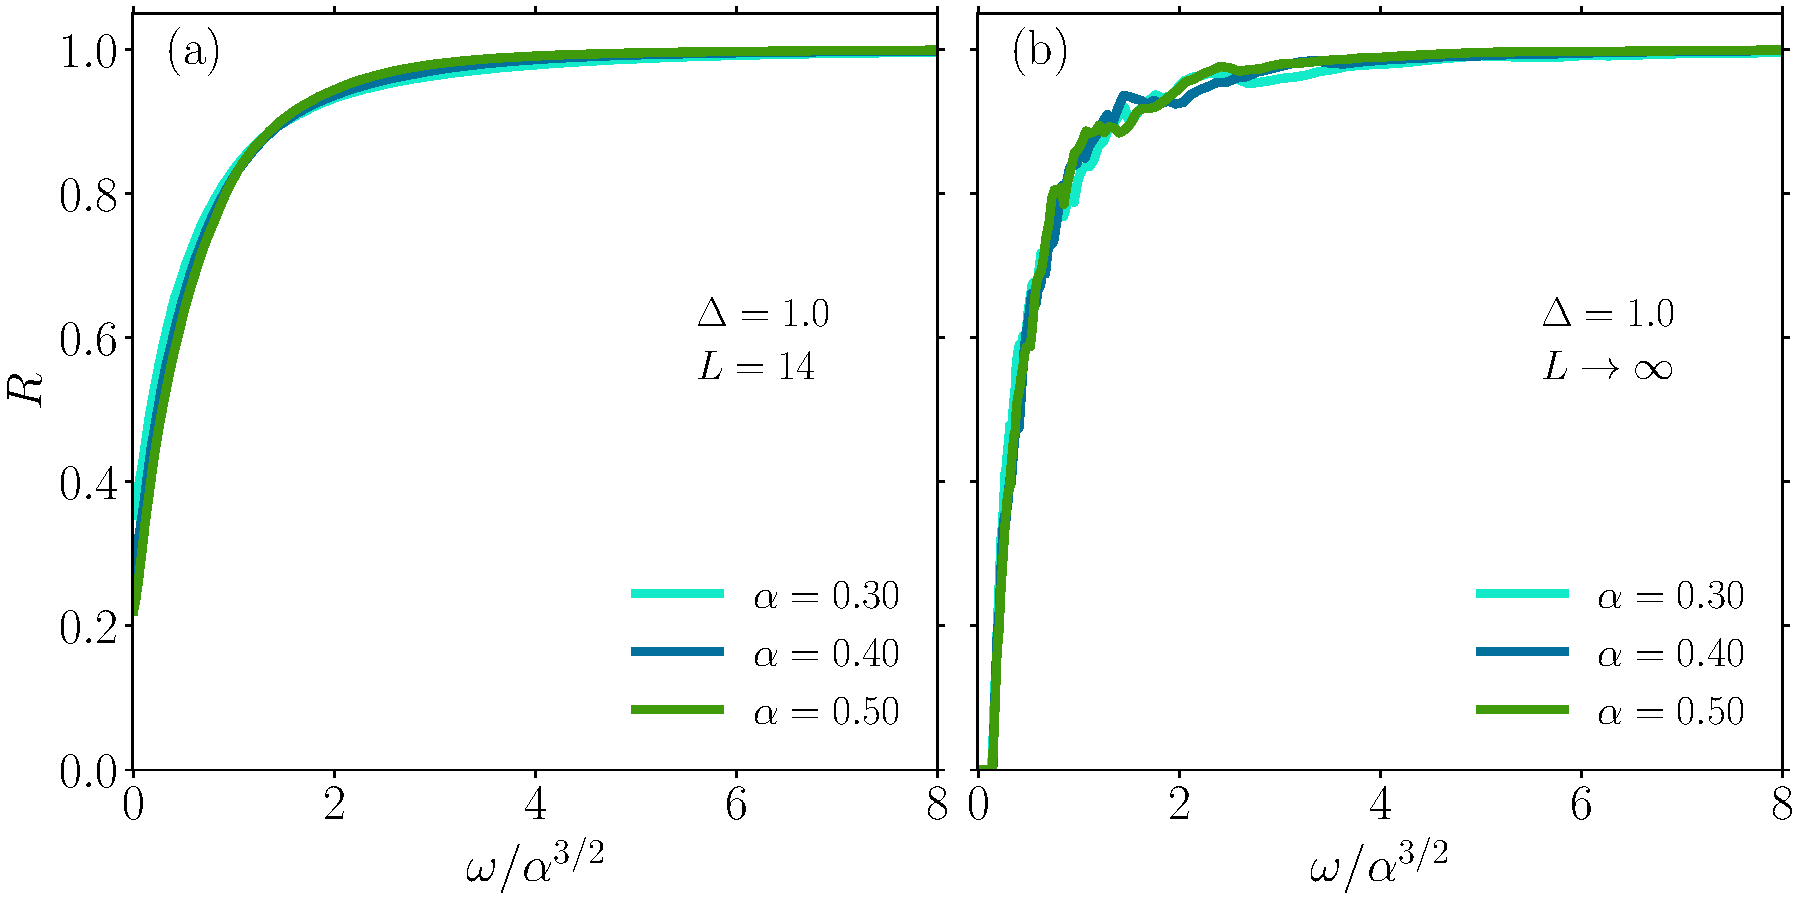
\includegraphics[width=\figsize\textwidth]{Figures/current_perfect_scaling.pdf}
  \caption{Normalized integrated spectral function as a function of 
  rescaled cutoff frequency for \(J^E\). The rescaling coefficient is chosen so as to obtain the 
  best possible collapse of curves. (a) Results for \(L=14\). (b) Results extrapolated
   to thermodynamic limit from \(L=11,12,13,14\).}\label{fig:current decay perfect scaling}
\end{figure}


\subsection{Relaxation of noncommuting (Q)LIOMs}
Let us now proceed with the same analysis, but for the \(\hat{O}_1\)~\eqref{eq:delta 1.0} 
and \(\hat{O}_2\)~\eqref{eq:delta 0.5} operators. Once again we shall look at the largest
system size available to us, that is \(L = 16\), as well as the case of extrapolation
to thermodynamic limit from \(L = 10,12,14,16\). 
Figure~\ref{fig:O12 no scaling} shows
\(R_{\mu}(\omega,\alpha)\), where \(\mu=1,2\), as a function of \(\omega\) for \(\alpha = 0.05,0.1,0.2\).
We have used weaker perturbations here, because Figure~\ref{fig:lioms decay} suggested that
it is enough to achieve vanishing stiffness in thermodynamic limit. Indeed this is the case
and we observe that \(\lim_{{\omega\to 0^{+}}} R_{\mu}(\omega,\alpha) = 0\) even for finite-size systems.
Basing on the discussion of energy current decay, next logical step would be to rescale the
frequency by \(\alpha^2\).
In contrast to the energy current, we not see any collapse (see Figure~\ref{fig:O12 quadratic scaling}).
Therefore, noncommuting operators do not follow the same universal scaling~\eqref{eq:universal scaling current}
as the energy current. However, as shown in Figure~\ref{fig:O12 linear scaling},
it turns out that a reasonable collapse, working for both \(\hat{O}_1\) and \(\hat{O}_2\),
may be observed for a different scaling, namely \(\omega/\alpha\). This suggests another kind
of relation:
\begin{equation}
  R_{\mu}(\omega,\alpha) \simeq \tilde{R}_{\mu}(\omega/\alpha)
\end{equation}
Moreover, the collapsed curves can be accurately fitted with an one-parameter error function
 (black dashed line in Figure~\ref{fig:O12 linear scaling}):
\begin{equation}
  \tilde{R}_{\mu}(\omega/\alpha) \simeq \erf\left(\frac{\omega}{\gamma \alpha}\right)
  \label{eq:erf fit}
\end{equation}
where the fitting parameter in denoted with \(\gamma\) and error function is defined as:
\begin{equation}
\erf(x) = \frac{2}{\sqrt{\pi}} \int_{0}^{x} \mathrm{d}t\; \mathrm{e}^{-t^2}  
\end{equation}
This implies a Gaussian, instead of
exponential, decay of autocorrelation function, i.e.\ \(\hs{\hat{O}_{\mu}(t)}{\hat{O}_{\mu}}
\propto \exp(-(t/\tau_{\mu})^2)\). We can once again make use of integrated spectral function
to see that this is correct.
\begin{align}
  S(\omega) &\propto \frac{1}{2\pi} \int_{-\infty}^{\infty} \mathrm{d}t \; \mathrm{e}^{-(t/\tau_{\mu})^2}
  \mathrm{e}^{i\omega t} = \frac{1}{2\pi} \int_{-\infty}^{\infty} \mathrm{d}t \; 
  \exp\left(-\frac{1}{\tau_{\mu}^2} \left(t-\frac{i\omega\tau_{\mu}}{2}\right)^2 
  - \frac{\omega^2\tau_{\mu}^2}{4}\right) \nonumber \\
  &= \exp\left(- \frac{\omega^2\tau_{\mu}^2}{4}\right) \frac{1}{2\pi}
  \int_{-\infty+\frac{i\omega\tau_{\mu}}{2}}^{\infty+\frac{i\omega\tau_{\mu}}{2}} 
  \mathrm{d} z\; \exp\left(-\frac{z^2}{\tau_{\mu}^2}\right) \nonumber\\
  & \triangleq \exp\left(- \frac{\omega^2
  \tau_{\mu}^2}{4}\right) \frac{1}{2\pi} \int_{-\infty}^{\infty}
  \mathrm{d} z\; \exp\left(-\frac{z^2}{\tau_{\mu}^2}\right) \nonumber  \\
  &= \frac{\tau_{\mu}}{2\sqrt{\pi}}\mathrm{e}^{-(\omega \tau_{\mu}/2)^2}
\end{align}
where between first and second line a change of variables \(z = t-\frac{i \omega \tau_{\mu}}{2}\)
has been made, and equality marked with \(\triangleq\) can be justified by means of contour
integration~\autocite{Stein2010}. Now we can easily perform integration over a finite
frequency window:
\begin{align}
  I(\omega) &\propto \frac{\tau_{\mu}}{2\sqrt{\pi}}\int_{-\omega}^{\omega} \mathrm{d}\omega^{\prime}\;
  \mathrm{e}^{-(\omega/\tau_{\mu})^2} = \frac{\tau_{\mu}}{2\sqrt{\pi}}
  \left[\int_{-\omega}^{0} \mathrm{d}\omega^{\prime} \mathrm{e}^{-(\omega\tau_{\mu}/2)^2} + 
  \int_{0}^{\omega} \mathrm{d}\omega^{\prime} \mathrm{e}^{-(\omega\tau_{\mu}/2)^2} \right]\nonumber\\
  &= \frac{\tau_{\mu}}{2\sqrt{\pi}} \left[ \frac{2}{\tau_{\mu}}\int_{-\frac{\omega\tau_{\mu}}{2}}^{0} 
  \mathrm{d} x\;  \mathrm{e}^{-x^2} + \frac{2}{\tau_{\mu}}\int_{0}^{\frac{\omega\tau_{\mu}}{2}}
   \mathrm{d}x\; \mathrm{e}^{-x^2} \right]\nonumber\\ 
   &= \frac{1}{\sqrt{\pi}} \left[ \frac{\sqrt{\pi}}{2} \erf\left(\frac{\omega\tau_{\mu}}{2}\right) +
   \frac{\sqrt{\pi}}{2} \erf\left(\frac{\omega\tau_{\mu}}{2}\right) \right]\nonumber\\
    &= \erf\left(\frac{\omega\tau_{\mu}}{2}\right)
\end{align}
where between first and second lines a change of variables \(x=\omega\tau_{\mu}/2\) has been made.
We have thus obtained the desired result~\ref{eq:erf fit}. On the contrary to the case of energy
current, the scaling of decay rate is \(\frac{1}{\tau_{\mu}} \propto \alpha\). This Gaussian relaxation
of noncommuting integrals of motion under weak perturbation is the main finding of this work.
One may ask a question about the origin of this anomalous scaling of characteristic time
\(\tau\). As noted in Subsection~\ref{subsec:noncomm qlioms}, operators exhibiting such scaling
are closely related to the massive degeneracies in energy spectrum of \(H_{XXZ}\) for
anisotropy  \(\Delta=1.0\) and \(\Delta = 0.5\), which is caused by states with
different total magnetization \(\Sz_{tot}\) but
equal energies. This in turn, is caused by certain symmetries of the Hamiltonian, simple \(SU(2)\) for
the former case and much more complex \(U_q(\mathfrak{sl}_2)\) for the latter 
case~\footnote{Technically, this symmetry is present only for \(\Delta=-0.5\), but this
can be amended in thermodynamic limit for chains of even length, as discussed in 
Subsection~\ref{subsec:noncomm qlioms}. }. 
When adding perturbation~\eqref{eq:perturbation}, there are actually two mechanism at play. We break
integrability while simultaneously breaking symmetry and thus lifting the macroscopic degeneracy.
We can disentangle these two mechanism, by studying behavior of \(\hat{O}_1\) and \(\hat{O}_2\)
under a different perturbation, namely:
\begin{equation}
  H^{\prime\prime} = \delta \sum_{j=1}^{L} \Sz_j \Sz_{j+1}
\end{equation}
This is equivalent to the unperturbed Hamiltonian for \(\Delta^{\prime} = \Delta + \delta\),
and allows us to eliminate degeneracy while preserving integrability. Results of this procedure
are shown in Figure~\ref{fig:O12 symmetry}. We see almost the same behavior as for system
with weakly broken integrability, i.e.\ the relaxation is Gaussian in nature with the
characteristic decay rate inversly proportional to \(\delta\). It is not the lack of
integrability but lack of symmetry-related degeneracy, occurring for either \(\alpha\neq 0\)
or \(\delta\neq 0\), that leads to this anomalous scaling.
\begin{figure}[ht]
  \centering
  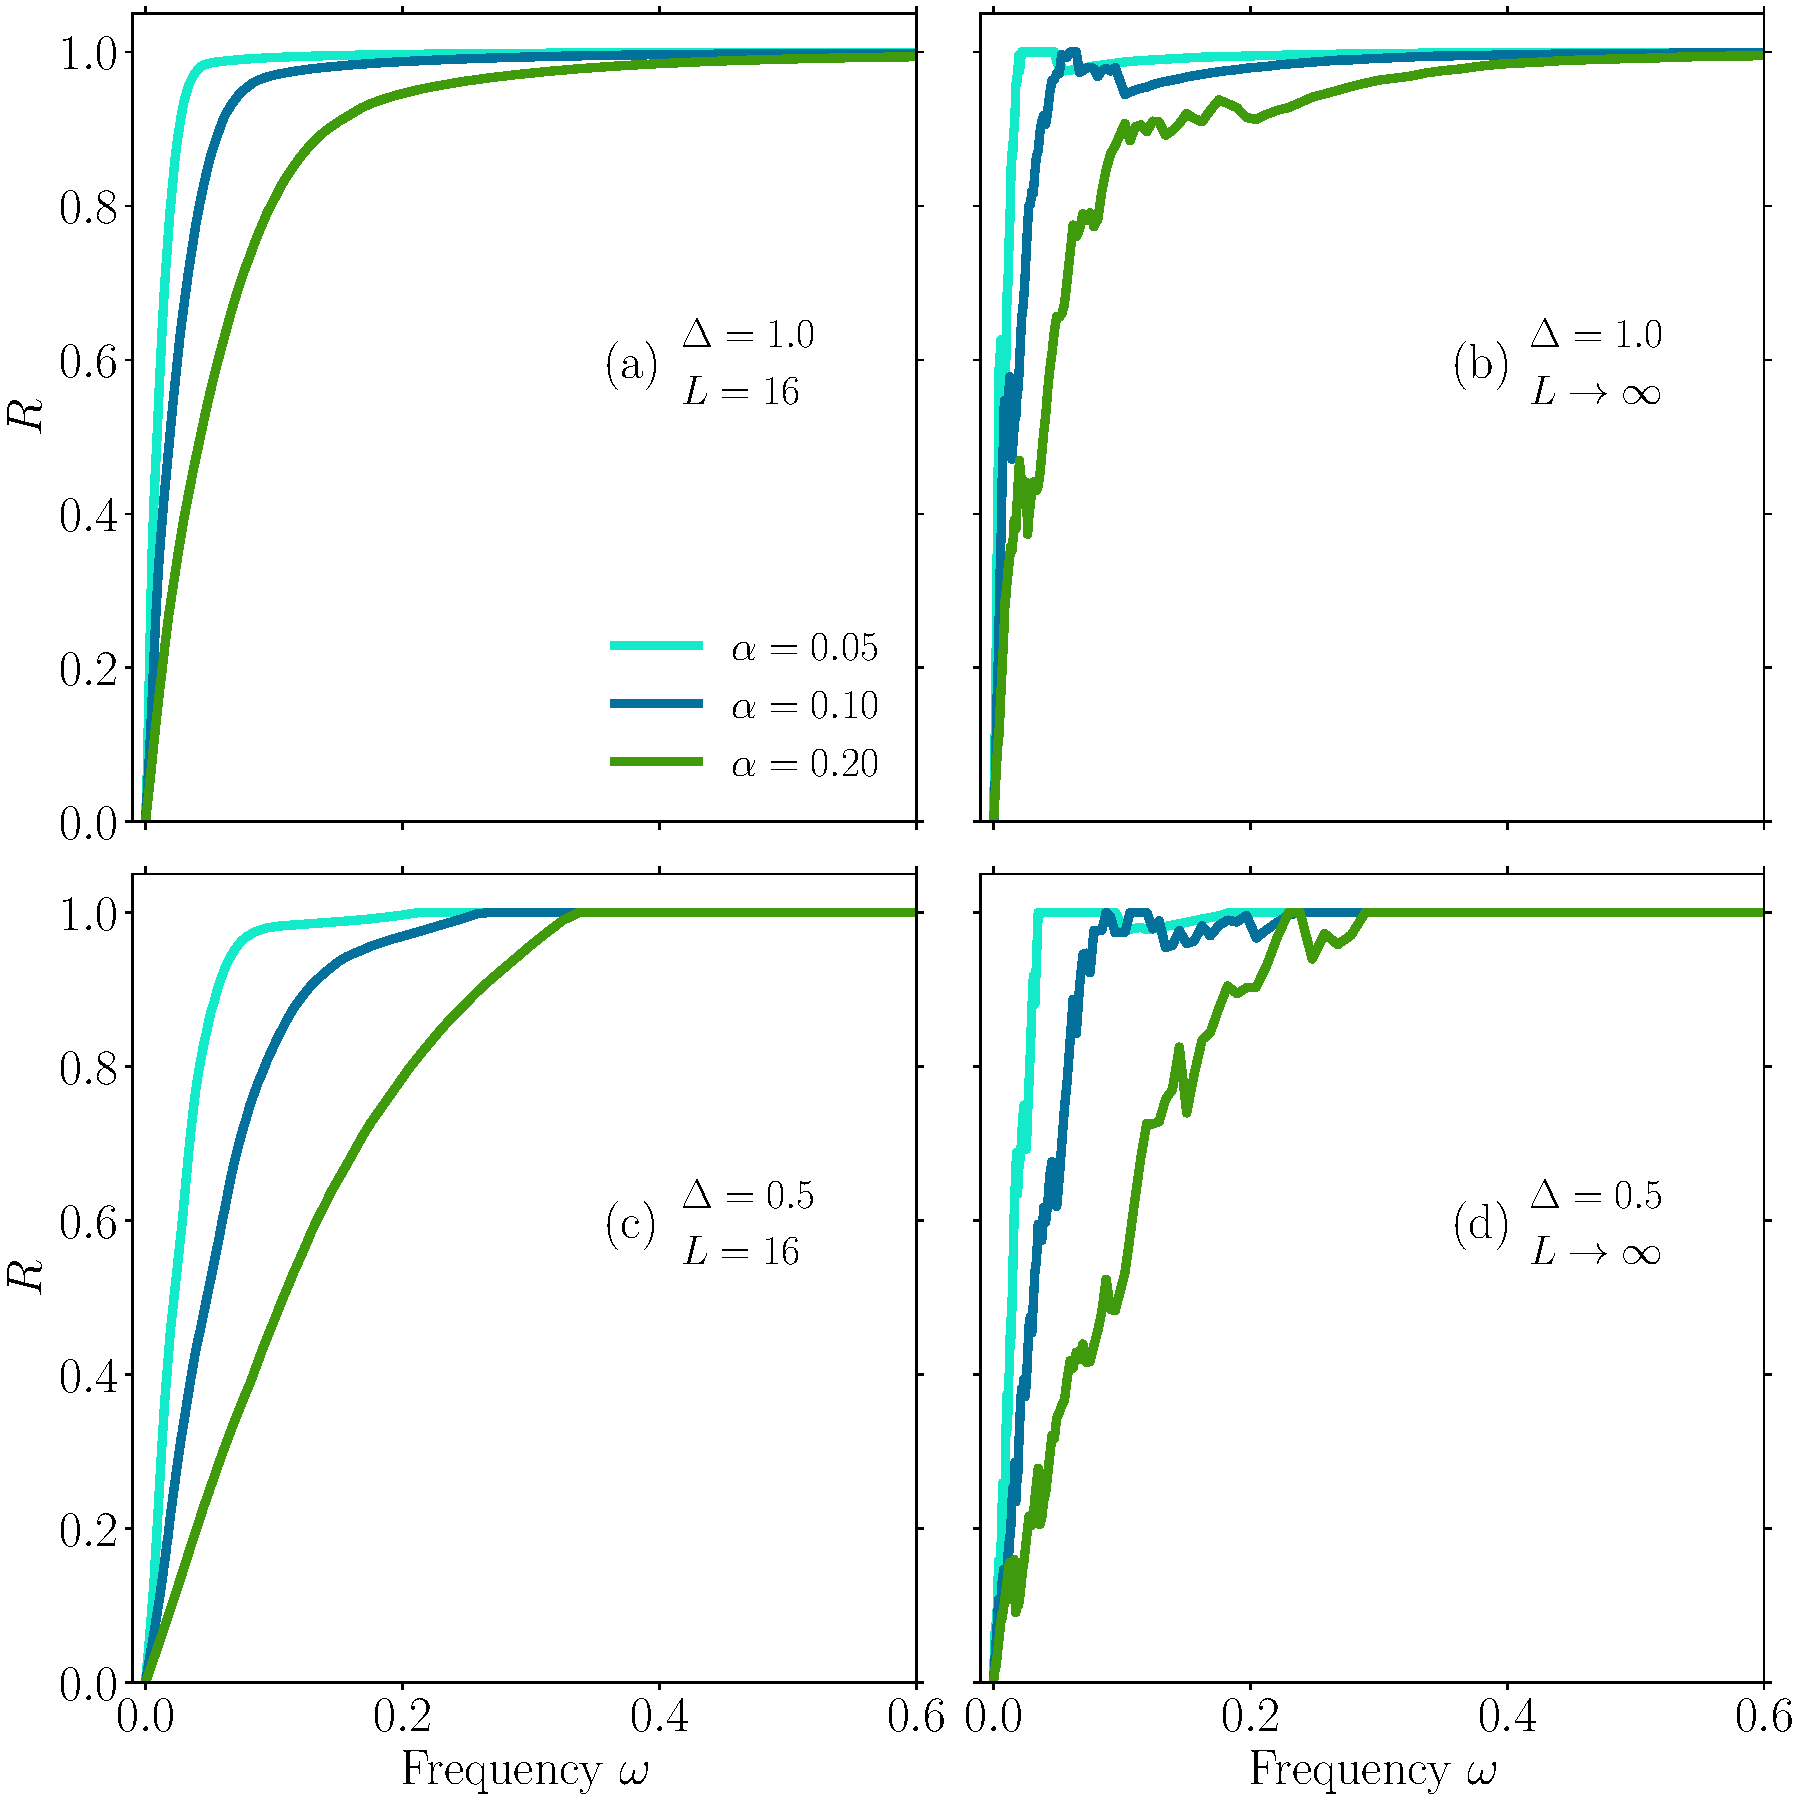
\includegraphics[width=\figsize\textwidth]{Figures/O12_no_scaling.pdf}
  \caption{Normalized integrated spectral function as a function of cutoff frequency for
  \(\hat{O}_1\) and \(\hat{O}_2\).
  (a) Results for \(L=16\) and \(\hat{O}_1\).  (b) Results for \(\hat{O}_1\) extrapolated to
  thermodynamic limit from \(L=10,12,14,16\). (c) Results for \(L=16\) and \(\hat{O}_2\). 
  (d) Results for \(\hat{O}_2\) extrapolated to thermodynamic limit from \(L=10,12,14,16\).
  Note that low frequency limit for finite system does approach \(0\), as expected from 
  Figure~\ref{fig:lioms decay}.
  }\label{fig:O12 no scaling}
\end{figure}
\begin{figure}[ht]
  \centering
  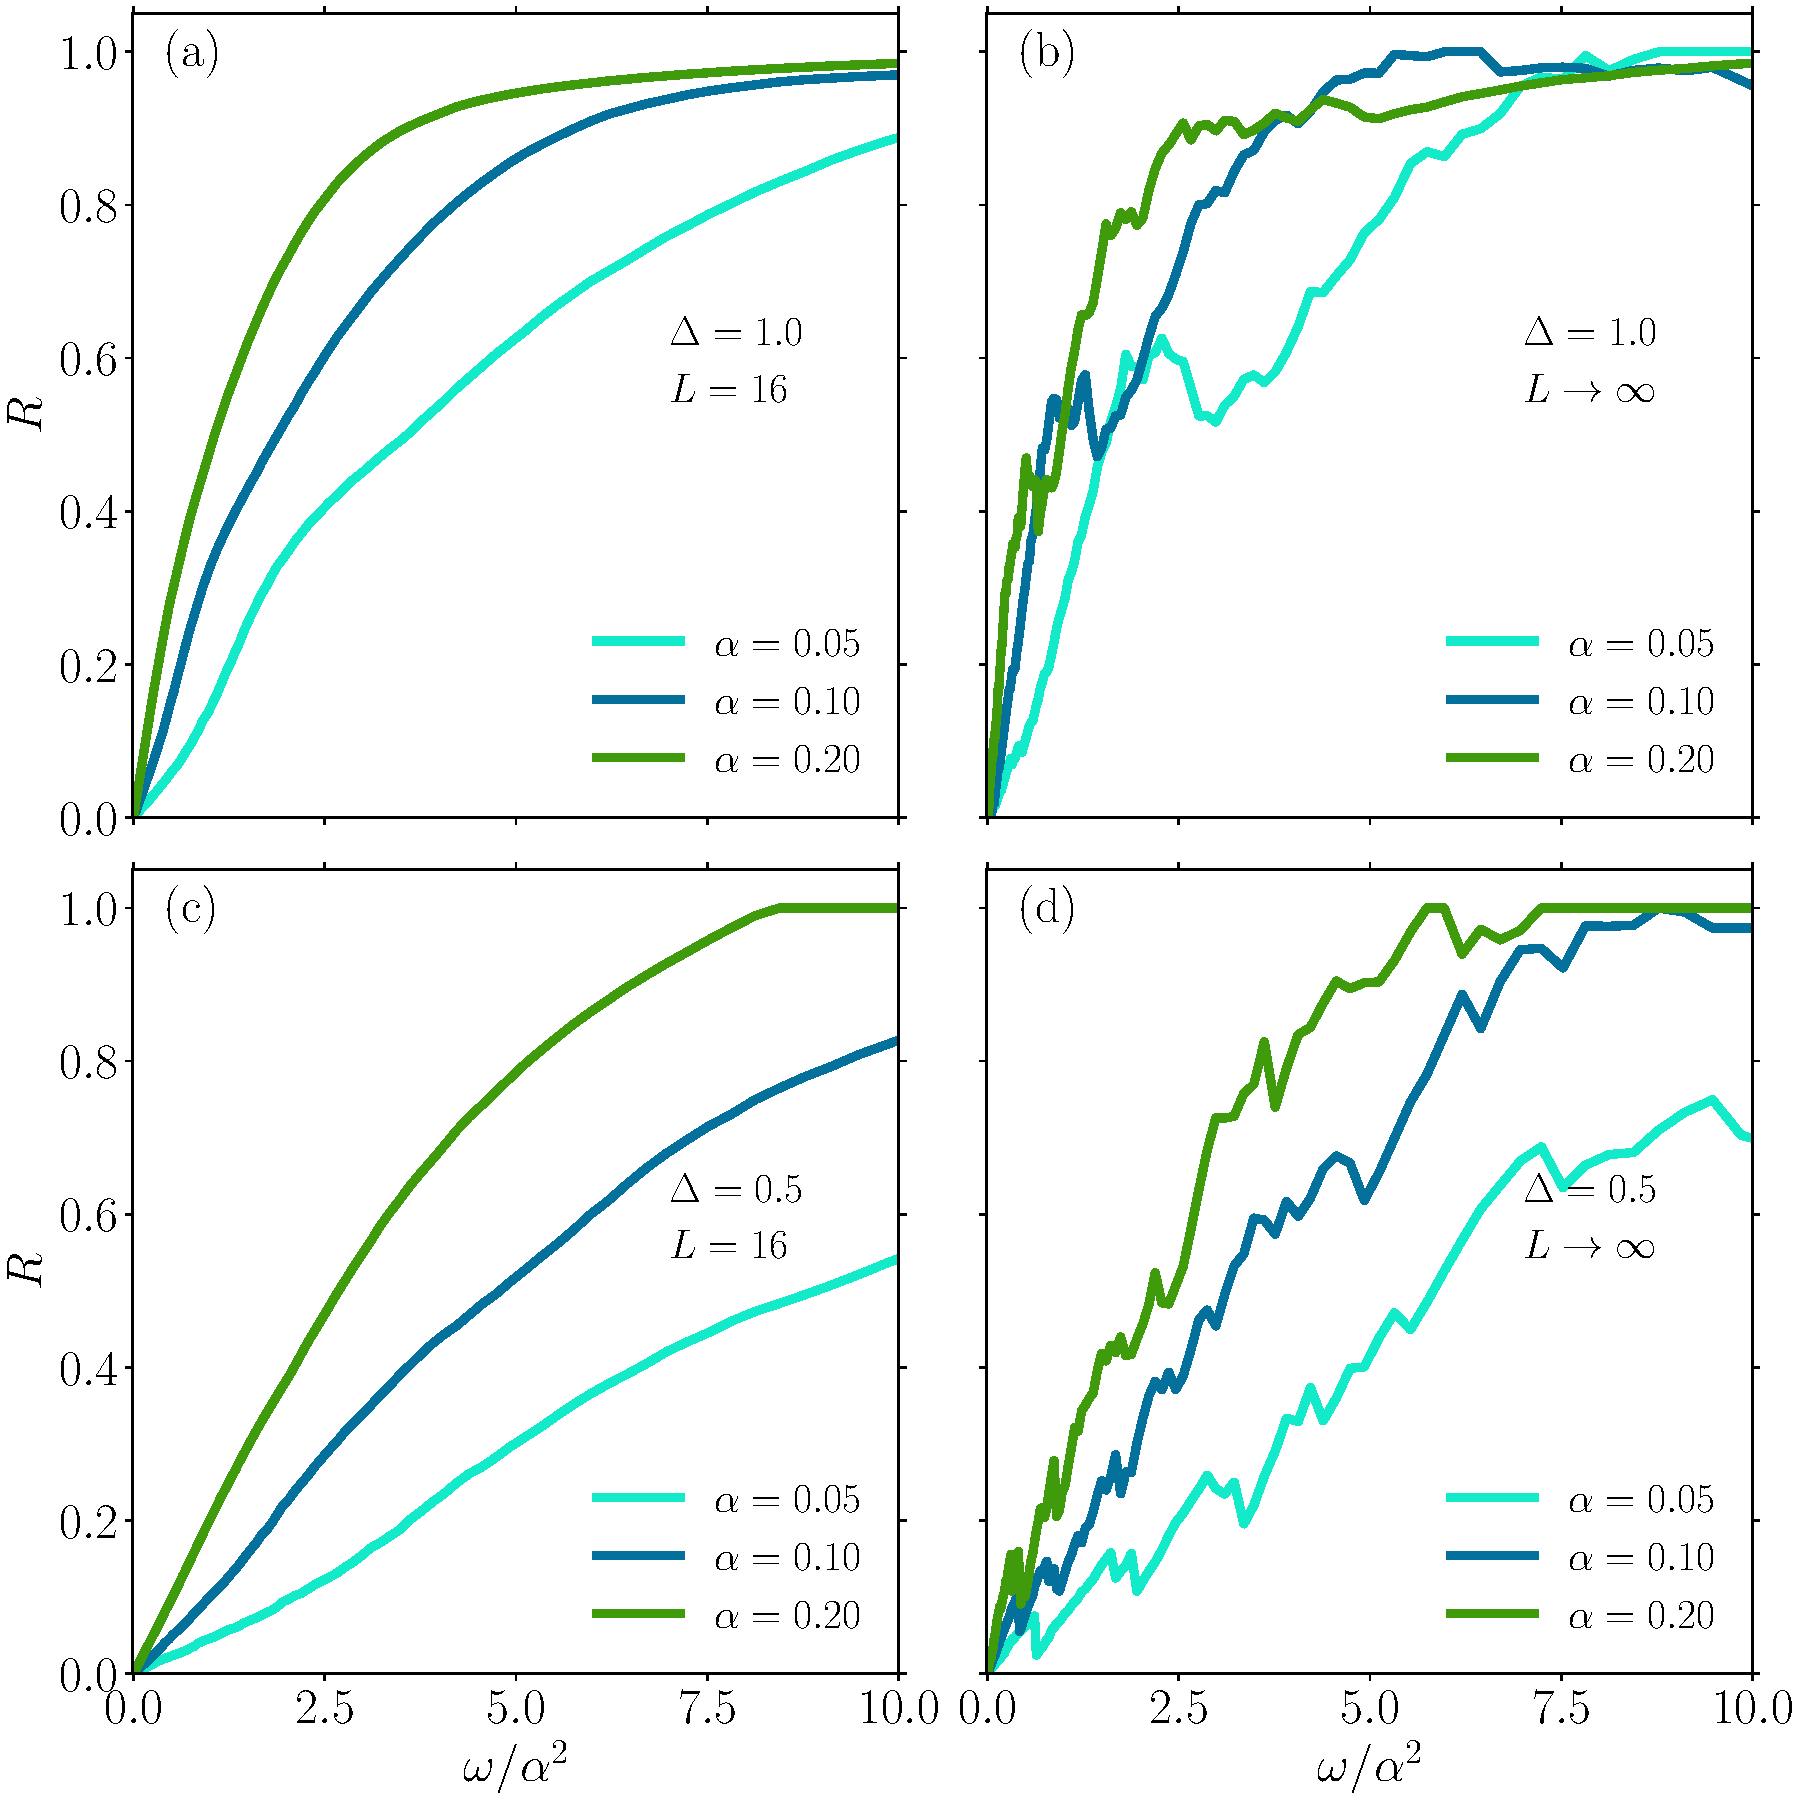
\includegraphics[width=\figsize\textwidth]{Figures/O12_quadratic_scaling.pdf}
  \caption{Normalized integrated spectral function as a function of rescaled 
  frequency \(\omega/\alpha^2\) for\(\hat{O}_1\) and \(\hat{O}_2\).
  (a) Results for \(L=16\) and \(\hat{O}_1\).  (b) Results for \(\hat{O}_1\) extrapolated to
  thermodynamic limit from \(L=10,12,14,16\). (c) Results for \(L=16\) and \(\hat{O}_2\). 
  (d) Results for \(\hat{O}_2\) extrapolated to thermodynamic limit from \(L=10,12,14,16\).
  On the contrary to the energy current, the curves do not collapse.}\label{fig:O12 quadratic scaling}
\end{figure}
\begin{figure}[ht]
  \centering
  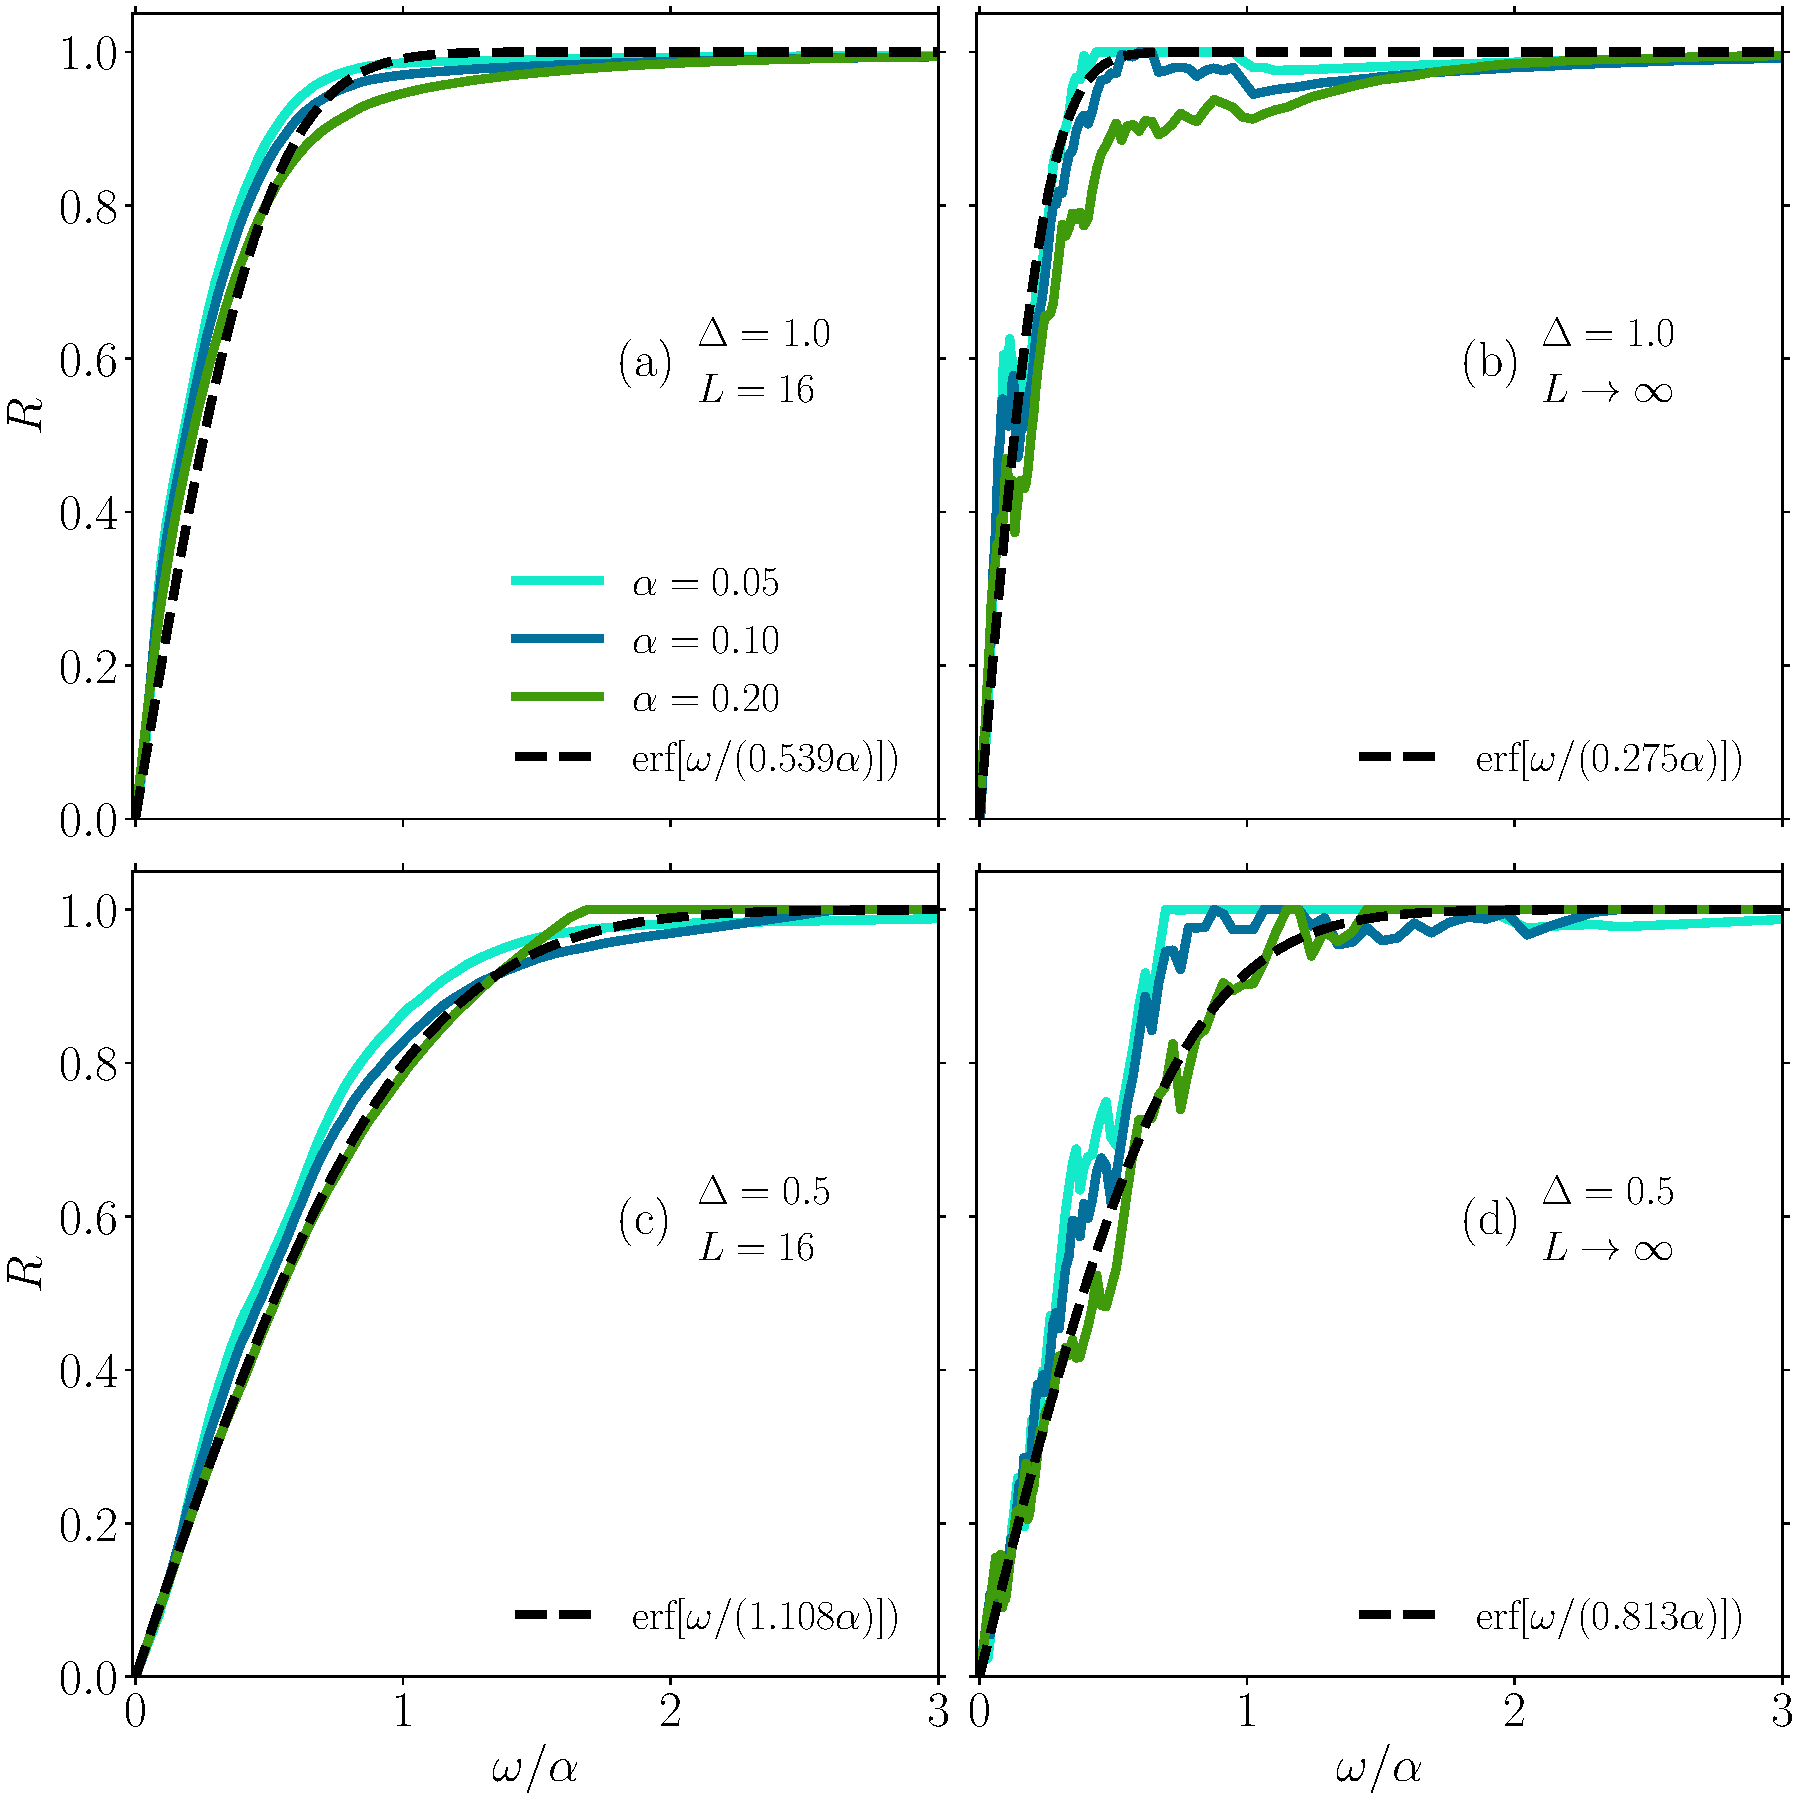
\includegraphics[width=\figsize\textwidth]{Figures/O12_linear_scaling.pdf}
  \caption{Normalized integrated spectral function as a function of rescaled 
  frequency \(\omega/\alpha\) for\(\hat{O}_1\) and \(\hat{O}_2\).
  (a) Results for \(L=16\) and \(\hat{O}_1\).  (b) Results for \(\hat{O}_1\) extrapolated to
  thermodynamic limit from \(L=10,12,14,16\). (c) Results for \(L=16\) and \(\hat{O}_2\). 
  (d) Results for \(\hat{O}_2\) extrapolated to thermodynamic limit from \(L=10,12,14,16\).
  Note the convincing collapse of the curves for this scaling.}\label{fig:O12 linear scaling}
\end{figure}
\textcolor{blue}{what about first-order perturbation theory?}
\begin{figure}[htbp]
  \centering
  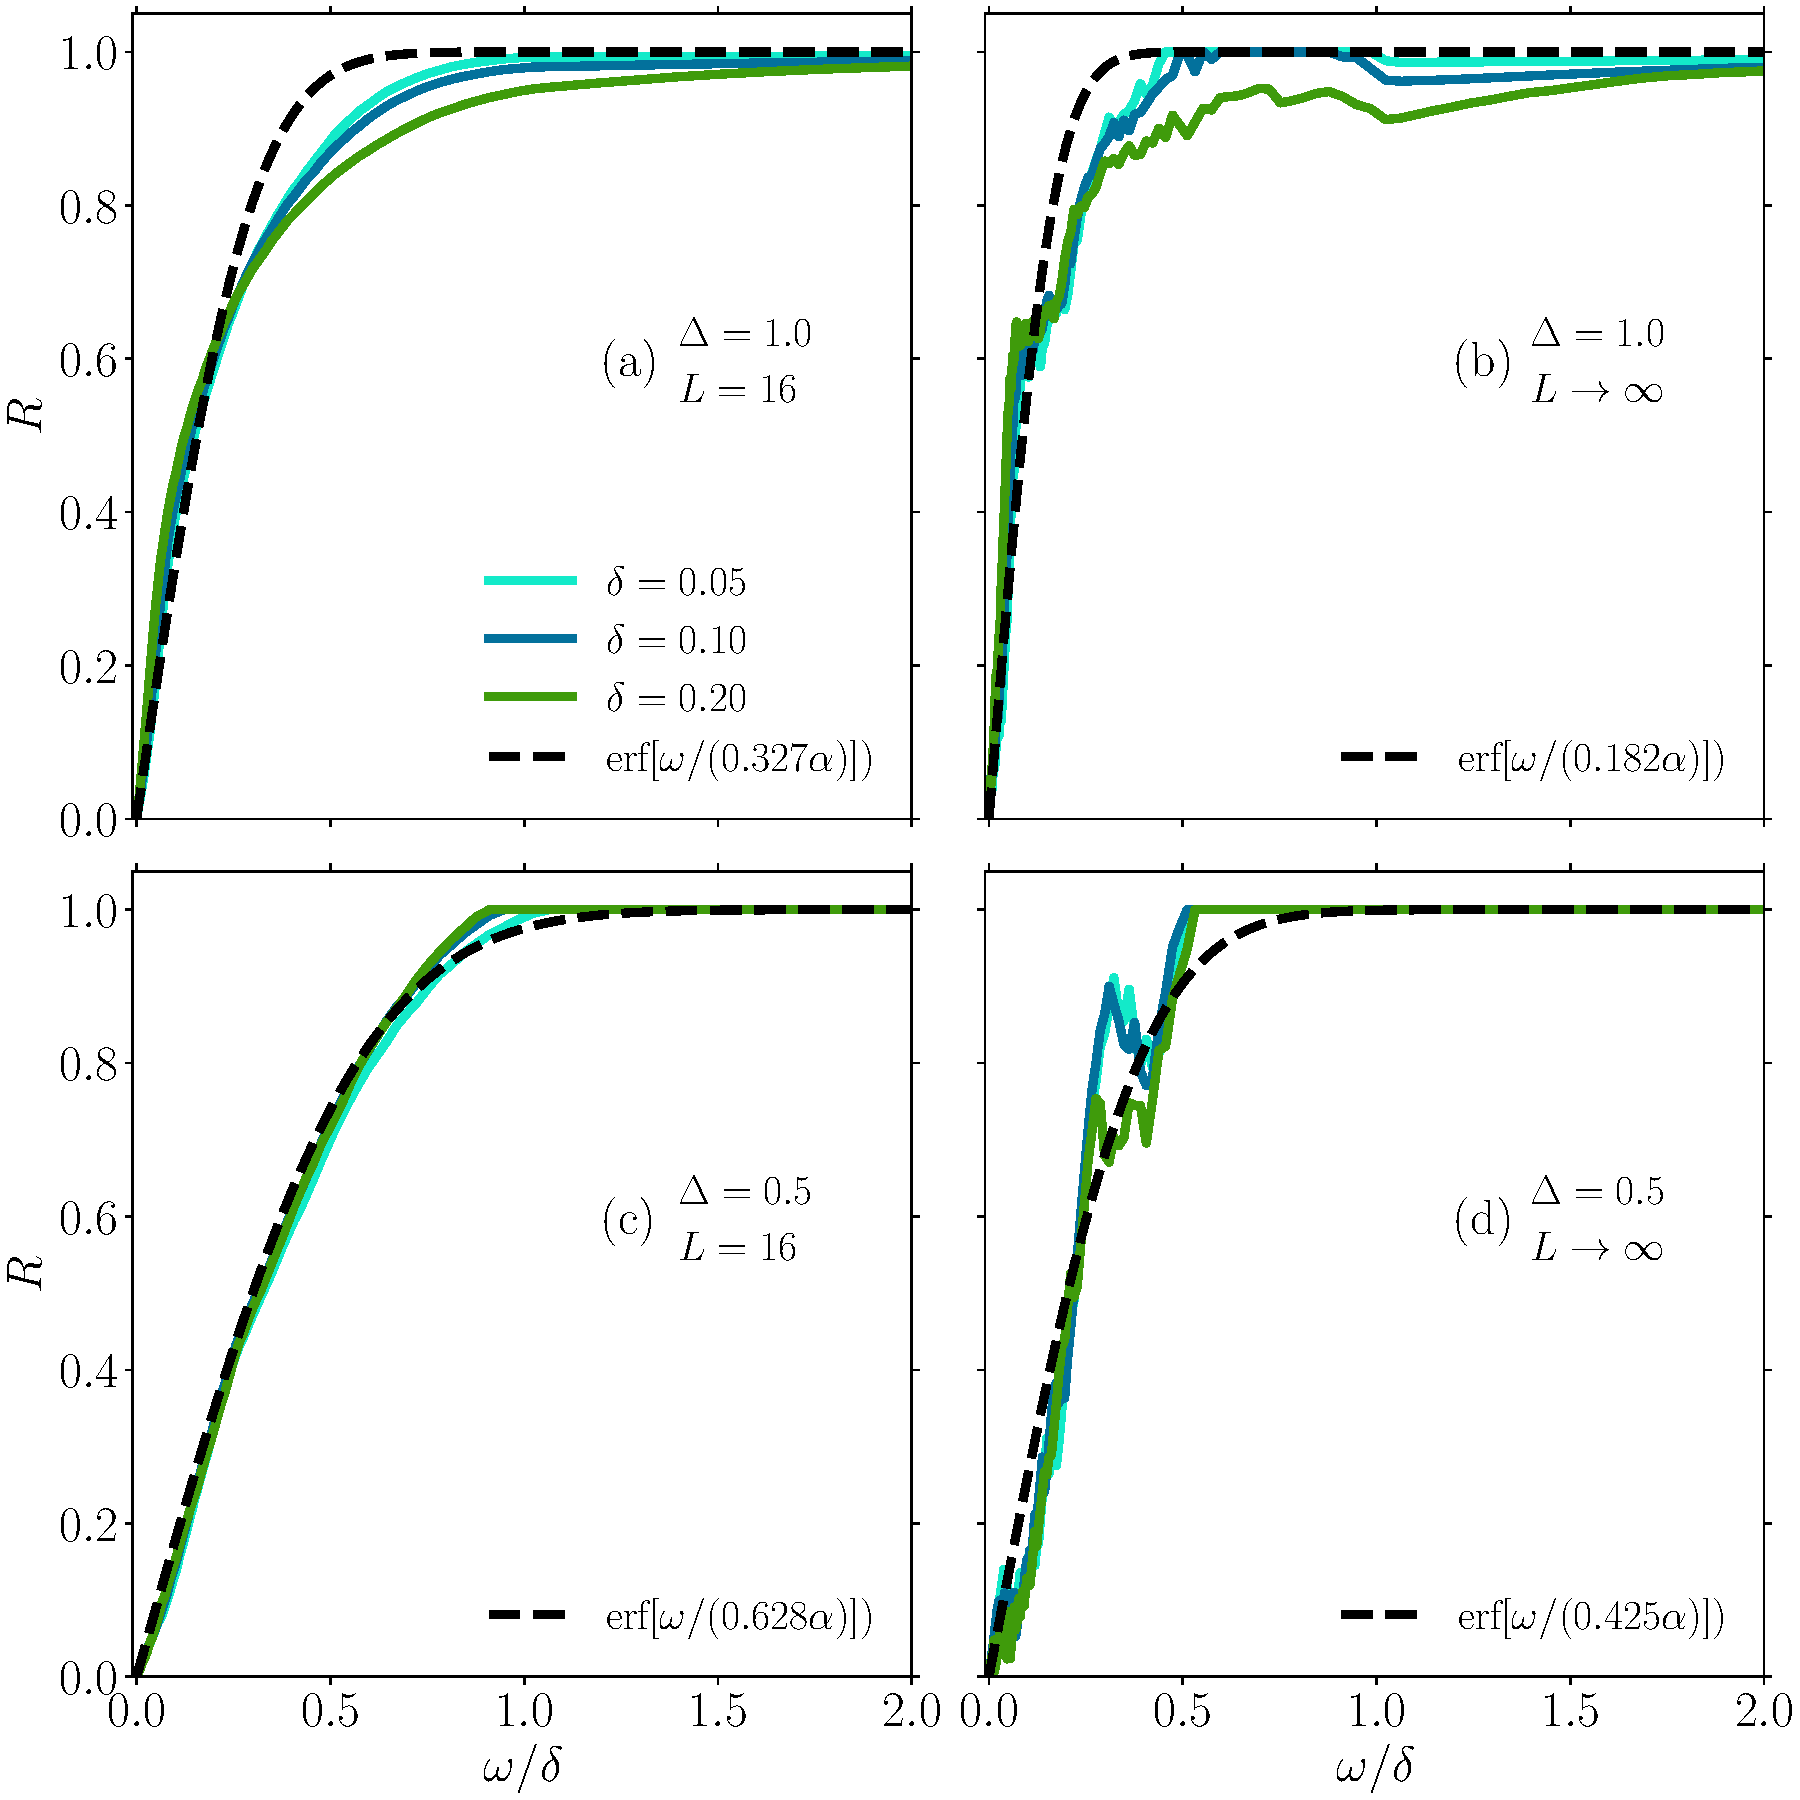
\includegraphics[width=\figsize\textwidth]{Figures/O12_symmetry_breaking.pdf}
  \caption{Normalized integrated spectral function as a function of rescaled 
  frequency \(\omega/\delta\) for\(\hat{O}_1\) and \(\hat{O}_2\). Here the model remains
  integrable, it only the symmetry that is broken.
  (a) Results for \(L=16\) and \(\hat{O}_1\).  (b) Results for \(\hat{O}_1\) extrapolated to
  thermodynamic limit from \(L=10,12,14,16\). (c) Results for \(L=16\) and \(\hat{O}_2\). 
  (d) Results for \(\hat{O}_2\) extrapolated to thermodynamic limit from \(L=10,12,14,16\).
  Results are qualitatively similar to full integrability breaking case. }\label{fig:O12 symmetry}
\end{figure}
